\chapter{Esempi}  \label{Cap.3}

\vspace{2cm}

\begin{flushright}
 \textit{Altri esempi di scrittura in \LaTeX\\ che non è stato possibile inserire nei capitoli precedenti.}
\end{flushright}

\vspace{0.5cm}

\section{listings}
Uso del pacchetto {\ttfamily listings} per la visualizzazione di codice Python:
\begin{lstlisting}[language=Python]
import numpy as np

def incmatrix(genl1,genl2):
    m = len(genl1)
    n = len(genl2)
    M = None #to become the incidence matrix
    VT = np.zeros((n*m,1), int)  #dummy variable

    #compute the bitwise xor matrix
    M1 = bitxormatrix(genl1)
    M2 = np.triu(bitxormatrix(genl2),1)

    for i in range(m-1):
        for j in range(i+1, m):
            [r,c] = np.where(M2 == M1[i,j])
            for k in range(len(r)):
                VT[(i)*n + r[k]] = 1;
                VT[(i)*n + c[k]] = 1;
                VT[(j)*n + r[k]] = 1;
                VT[(j)*n + c[k]] = 1;

                if M is None:
                    M = np.copy(VT)
                else:
                    M = np.concatenate((M, VT), 1)

                VT = np.zeros((n*m,1), int)

    return M
\end{lstlisting}


\section{Testo multicolonna}

\begin{multicols}{2}
    \textbf{Colonna 1}\\
    Testo della prima colonna.\\
    Lorem ipsum dolor sit amet, consectetuer adipiscing elit. Etiam lobortis facilisis sem.
    \columnbreak\\
    \textbf{Colonna 2}\\
    Testo della seconda colonna.\\
    Lorem ipsum dolor sit amet, consectetuer adipiscing elit. Etiam lobortis facilisis sem. Nullam nec mi et neque pharetra sollicitudin. Praesent imperdiet mi nec ante. Donec ullamcorper, felis non sodales commodo, lectus velit ultrices augue, a dignissim nibh lectus placerat pede.
\end{multicols}

\newpage
\section{Spazi e ritorni}
{\ttfamily \textbackslash newpage} termina la pagina attuale e inizia una nuova pagina.

Segue uno spazio vuoto di 2cm.

\vspace*{2cm}

Per forzare uno o più spazi bisogna usare uno o più backslash, ognuno seguito da uno spazio.\\
Testo normale\\
Testo \ con uno spazio in più\\
Testo \ \ con due spazi in più\\
Testo \ \ \ con tre spazi in più\\

Per forzare \LaTeX\ ad inserire una nuova riga vuota, inserire uno spazio e poi andare a capo.\\
\begin{verbatim}
\ \\
\end{verbatim}
Per scrivere questa sezione è stato usato il blocco {\ttfamily verbatim}, il testo al suo interno non viene
interpretato in alcun modo.



Un elenco di elenchi??

Roba degna del più famoso elencatore d'Italia.
\begin{itemize}
    \item Dell'aria
    \item Dell'acqua
    \item Dei fiumi
    \item Dei mari
    \item dei nostri boschi
    \item delle nostre montagne
    \item dei nostri ghiacciai
    \begin{itemize}
        \item puliti
        \item riciclabili
        \item rinnovabili
        \item biodegradabili
    \end{itemize}
\end{itemize}





\newpage
\begin{landscape}
    \section{Testo orizzontale}
    landscape ruota il contenuto della pagina in orizzontale.

    Per scrivere un'equazione su \LaTeX si può ricorrere a molteplici modi:
    \begin{itemize}
        \item $F=ma$
        \item Per centrare l'equazione:
        \[E=mc^2\]
    \end{itemize}
    Se si vuole numerare e centrare l'equazione si procede in questo modo:
    \begin{equation}
        F=ma
    \end{equation}

\end{landscape}

\section{Immagini e tabelle}

Per inserire due immagini sotto la stessa didascalia bisogna seguire il seguente iter:

\begin{figure}
    \centering
    \subfloat[][\emph{Immagine 1}]
    {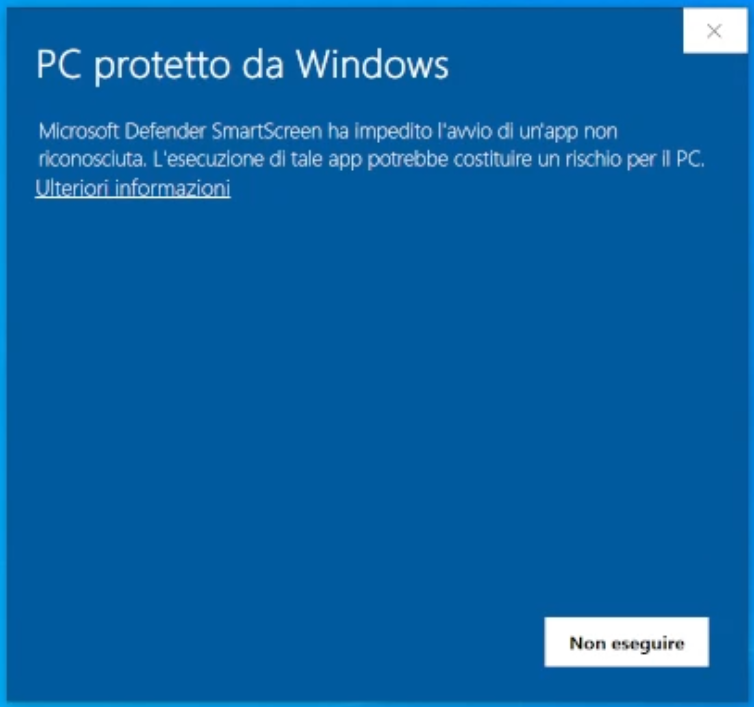
\includegraphics[width=.4\textwidth]{01_images/texlive/win/1_smart_screen.png}} \quad
    \subfloat[][\emph{Immagine 2}]
    {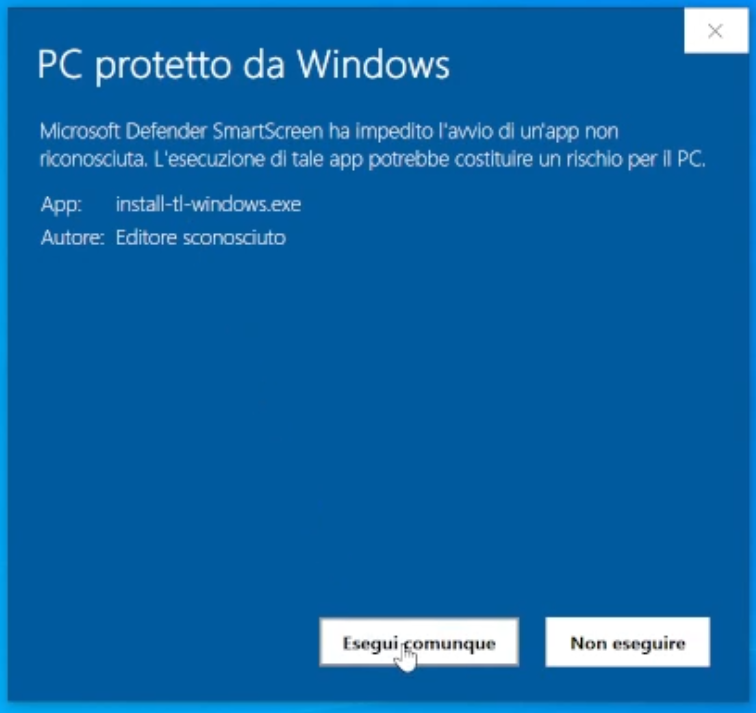
\includegraphics[width=.4\textwidth]{01_images/texlive/win/2_smart_screen_2.png}} \\
\caption{Due immagini di prova}
\label{struttura}
\end{figure}

\begin{table}[!ht]
    \centering
    \caption{ESEMPIO}
    \begin{tabular}{llll}
    \hline
        ESEMPIO & 1 & 2 & 3 \\ \hline
        A & A1 & A2 & A3 \\
        B & B1 & B2 & B3 \\
        C & C1 & C2 & C3 \\ \hline
    \end{tabular}
    \label{ESEMPIO}
\end{table}

Approfondimento sul posizionamento delle immagini \citep{forceFigurePlacement}

\section{Scorciatoie e consigli}

Ecco alcune indicazioni per ottimizzare al meglio il tuo documento:

\begin{itemize}
    \item Se il documento è molto lungo e ci metti tanto tempo
    per risalire al codice ma hai il pdf aperto,
    fai Ctrl+click (pulsante sx del mouse) sul testo che cerchi nel pdf.
    \item se vuoi scrivere una formula matematica in grassetto, con all'interno simboli, vanno utilizzati
    i comandi $mathbf$ e $boldsymbol$. Ecco un esempio: $\mathbf{a=\boldsymbol{\Gamma}^{-1}u}$.
    \item Per costruire tabelle in modo più rapido utilizza il seguente link: \url{https://tableconvert.com/it/excel-to-latex}
\end{itemize}
